\section{Introduction}

% ¶1 宏观背景铺垫
Latency-sensitive, single-request serving dominates interactive LLM applications such as chat assistants, code completion, and knowledge retrieval. Mixture-of-Experts (MoE) architectures have been increasingly gaining traction for powering such workloads~\cite{lepikhin2021gshard,fedus2022switch,rajbhandari2022deepspeed}, scaling model capacity without proportionally increasing per-token compute; frontier open-weight models such as Qwen3, Mixtral, and DeepSeek-V3 all adopt this paradigm. However, the sheer number of experts makes their aggregate memory footprint far exceed the capacity of commodity accelerators. Speculative decoding (SD) is the standard technique for reducing autoregressive decode latency, routinely delivering $2$--$3\times$ speedup on dense models~\cite{leviathan2023fast,chen2023accelerating,li2024eagle,li2025eagle3}. Whether SD remains effective when MoE models cannot fit entirely in GPU memory, however, is an open question.

% ¶2 具体场景 + SD失败机制
To investigate, consider a developer running a chat assistant powered by Qwen3-30B-A3B on a workstation with one 46~GB GPU. The model's 128 experts per layer require about 57.6~GB in bf16, exceeding the GPU budget. The standard remedy is Unified Virtual Addressing (UVA), which places expert weights in host memory and loads them on demand via PCIe. As Figure~\ref{fig:motivation} illustrates, SD is surprisingly ineffective under UVA: it yields only $1.17\times$ speedup. The reason is not a weak draft model. Rather, multi-token verification expands the per-layer expert working set from $\war=8$ to $\wsd\approx 19.3$ (up to 26.9), amplifying PCIe transfer by $2.4\times$ and keeping expert access in the PCIe-bound regime. In other words, SD fails because it makes the memory bottleneck \emph{worse}, not because it lacks algorithmic advantage.

\begin{figure}[t]
\centering
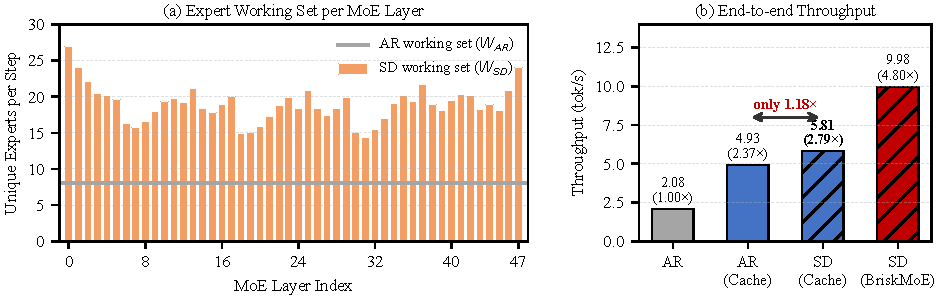
\includegraphics[width=\columnwidth]{figures/fig_motivation.pdf}
\caption{Motivating profiling. (a)~SD expands the per-layer expert working set from $\war=8$ to an average of $\wsd\approx 19.3$ (up to 26.9), amplifying PCIe transfer by $2.4\times$. (b)~End-to-end throughput: SD alone yields only $1.17\times$, but \sysname reaches $4.80\times$ by switching expert access from PCIe to HBM.}
\Description{Panel a shows a bar chart of 48 MoE layers comparing AR working set of 8 with SD working set ranging from 14 to 27. Panel b shows a 4-way grouped bar chart at 44 GB where SD plus BriskMoE reaches 9.98 tokens per second.}
\label{fig:motivation}
\end{figure}

% ¶3 现有工作局限
Existing works do not effectively address this problem due to three gaps. (1)~Analytical studies of SD on offloaded MoE adopt a batch-centric model in which every layer loads the complete expert set, making SD unconditionally beneficial through increased arithmetic intensity~\cite{liu2025specmoeoffload}. This model does not apply to single-request serving, where each layer activates only a small subset of experts and SD's working-set expansion translates into proportionally more PCIe transfer rather than higher compute utilization. (2)~Uncached offloading mechanisms such as UVA expose every expert access to PCIe without regard to temporal locality. They provide no caching layer to absorb repeated accesses, so the enlarged working set under SD compounds the PCIe cost with no way to mitigate it. (3)~Cache-based MoE systems such as MoE-Infinity~\cite{xue2024moeinfinity} and pre-gated MoE~\cite{hwang2023pregated} maintain GPU-resident expert caches to accelerate autoregressive decoding, but are designed for single-token inference. SD's multi-token verification step accesses a substantially wider set of experts per layer, causing rapid cache turnover that these systems neither anticipate nor handle. In particular, none of these works addresses the interplay between expert cache coverage and speculative verification that governs SD effectiveness under offloaded MoE serving.

% ¶4 Key insight + 提出方案 + 核心设计
The key insight behind our work is that the decisive optimization lever is not increasing arithmetic intensity but \emph{switching the bandwidth regime} of expert accesses---from PCIe ($\bpcie=25$~GB/s) to HBM ($\bhbm=768$~GB/s), a ratio of $30.7\times$ that dwarfs any arithmetic-intensity improvement achievable by SD alone. Based on this insight, this paper presents \sysname, a novel system for effective speculative decoding on latency-first, single-request offloaded MoE inference. \sysname is developed with three designs:
\begin{enumerate}[leftmargin=1.5em]
\item \textbf{Enable:} shift expert access from the PCIe-bound regime to the HBM-bound regime by allocating per-layer expert cache pools, guided by a bandwidth-regime model $\beff(\eta)=\eta\cdot\bhbm+(1-\eta)\cdot\bpcie$.
\item \textbf{Unblock:} once caching becomes effective, new bottlenecks emerge along the cache path---scratchpad copies, CPU-GPU synchronization, residual misses, and kernel inefficiency. \sysname removes them in sequence through four targeted mechanisms (Section~\ref{sec:design}).
\item \textbf{Protect:} SD enlarges the working set exactly when cache space is scarce. \sysname uses draft-guided preloading to maintain cache coverage under SD's expanded working set, preventing the system from falling back into the transition regime.
\end{enumerate}

% ¶5 贡献列举
In summary, this paper makes the following contributions.
\begin{itemize}[leftmargin=1.2em]
\item We present the first bandwidth-regime analysis of single-request offloaded MoE serving and identify a previously unreported phase transition in which SD is nearly useless (PCIe-bound), cache-pressured (transition), or highly effective (HBM-bound) (Section~\ref{sec:model}).
\item We develop \sysname, a novel system with three designs---Enable, Unblock, Protect---that makes SD an effective latency accelerator for offloaded MoE inference. \sysname is implemented as a non-intrusive vLLM plugin without modifying the core inference runtime (Section~\ref{sec:design}).
\item We conduct extensive experiments on Qwen3-30B-A3B with EAGLE-3 and show that \sysname achieves up to $4.80\times$ speedup over the offload baseline, restoring SD to a $1.36\times$ multiplier over cached autoregressive decoding at 44~GiB (Section~\ref{sec:eval}).
\end{itemize}

% ¶6 论文组织
The rest of the paper is organized as follows. Section~\ref{sec:background} introduces the serving scenario and notation. Section~\ref{sec:model} presents the bandwidth-regime analysis. Section~\ref{sec:design} describes the three-stage \sysname design. Section~\ref{sec:eval} reports experimental results. Section~\ref{sec:related} discusses related work and Section~\ref{sec:conclusion} concludes the paper.